\section{重建: \Egraph 不变量维护的全新视角}
% \section{Rebuilding: A New Take on \Egraph Invariant Maintenance}
\label{sec:rebuild}
\label{sec:rebuilding}

% Rebuilding is a new, general perspective on \egraph invariant maintenance.
% Traditionally~\cite{nelson, simplify},
%   \egraphs maintain their data structure invariants
%   after each operation.
% We separate this invariant restoration into a procedure called \textit{rebuilding}.
% This separation allows the client to
%   choose when to enforce the \egraph invariants.
% Performing a rebuild immediately after every operation replicates the
%   traditional approach to invariant maintenance.
% In contrast, rebuilding less frequently can amortize the cost of invariant
%   maintenance, significantly improving performance.
传统上~\cite{nelson, simplify},\egraphs 在每次操作后保持数据结构不变式。
我们将这种不变式恢复分为称为 \textit{rebuilding(重建)} 的过程。
这种分离允许客户端选择何时执行 \egraph 不变式。
立即在每次操作后执行重建就复制了传统的不变式维护方法,
相比之下,较少的重建可以摊销不变式维护成本,显著提高性能。

% In this section, we first describe how e-graphs have
%   traditionally maintained invariants (\autoref{sec:upward}).
% We then describe the rebuilding framework and how it captures a spectrum of
%   invariant maintenance approaches, including the traditional one
%   (\autoref{sec:rebuilding-detail}).
% Using this flexibility, we then give a modified algorithm for equality
%   saturation that enforces the \egraph invariants at only select points
%   (\autoref{sec:rebuilding-eqsat}).
% We finally demonstrate that this new approach offers an asymptotic speedup over
%   traditional equality saturation (\autoref{sec:rebuild-eval}).
在本节中,我们首先描述了 e-graphs 如何传统地维护不变量(\autoref{sec:upward})。
然后,我们描述了重构框架以及它如何捕获一系列维护不变量的方法,
  包括传统方法(\autoref{sec:rebuilding-detail})。
利用这种灵活性,我们然后给出了一种修改的算法,用于 等式饱和 ,
  它只在特定点强制执行 \egraph 不变量(\autoref{sec:rebuilding-eqsat})。  %?enforces the \egraph invariants
最后,我们证明这种新方法比传统的等价饱和提供了渐进加速 % ?asymptotic speedup
  (\autoref{sec:rebuild-eval})。



% 原文注释 begin
% Among \egg's optimizations (\autoref{sec:egg-efficient}),
%   strategically delayed rebuilding is perhaps the most important.
% \egg employed a m
% Delayed rebuilding amortizes the cost of invariant maintenance, significantly reducing work

% Rebuilding is a novel technique that lies at the heart of \egg's
%   modified equality saturation algorithm.
% This crucial technique allows equality saturation to specialize the \egraph to
%   its workload, yielding substantial performance improvements.
%   %from both an algorithmic and implementation
%   %perspective.

% Rebuilding gives the user (or algorithm) choice on when to restore the \egraph
%   invariants, which can have a large impact on performance .

% The key insight is that maintaining the \egraph invariants is expensive, and

% \autoref{fig:eq-sat-code} shows both the traditional and \egg's modified
%   equality saturation loop.
% The key distinction is \textit{when} the \egraph invariants of deduplication and
%   congruence are maintained.
% In traditional \egraphs, like with many data structures, invariants always
%   hold.
% In contrast, mutating an \egg \egraph may violate invariants, causing equalities
%   to be not ``seen'' when searching for patterns.
% \egg lets the user (or the algorithm) choose when to restore the invariants by
%   calling the \texttt{rebuild} method.
% Rebuilding leads to a lower amortized cost of maintaining the \egraph invariants.
% 原文注释 end

% \subsection{Upward Merging}
\subsection{向上合并}
\label{sec:upward}

% Both mutating operations on the \egraph
%   (\texttt{add} and \texttt{merge}, \autoref{sec:interface})
%   can break the \egraph invariants if not done carefully.
% \Egraphs have traditionally used \textit{hashconsing} and
%   \textit{upward merging} to maintain the congruence invariant.
如果不仔细操作,对 \egraph 进行的变异操作 (\texttt{add} 和 \texttt{merge},\autoref{sec:interface})
  可能会破坏 \egraph 不变性。
\Egraphs 传统上使用 \textit{哈希康化(hashconsing)} 和  % ?hashconsing
  \textit{向上合并(upward merging)} 来维护同余不变性。


% The \texttt{add} operation relies on the hashcons invariant
%   (Definition \ref{def:hash-inv})
%   to quickly check whether the \enode $n$ to be added---or one congruent to it---is
%   already present.
% Without this check, \texttt{add} would create a new \eclass with $n$ in it
%   even if some $n' \cong n$ was already in the \egraph,
%   violating the congruence invariant.
\texttt{add} 操作依赖于哈希康不变性 (hashcons invariant,定义 \ref{def:hash-inv}) 来
  快速检查要添加的 \enode $n$ 或与其同余的节点是否已经存在。
如果没有这个检查,\texttt{add} 将创建一个新的 \eclass,
  其中包含 $n$,即使某些 $n' \cong n$ 已经在 \egraph 中,这将违反同余不变性。


% The \texttt{merge} operation \eclasses can violate both \egraph invariants.
% If $f(a, b)$ and $f(a, c)$ reside in two different \eclasses $x$ and $y$,
%   merging $b$ and $c$ should also merge $x$ and $y$ to maintain the congruence invariant.
% This can propagate further, requiring additional merges.
\texttt{merge} 操作可能会违反 \egraph 的两个不变性。
如果 $f(a, b)$ 和 $f(a, c)$ 分别位于两个不同的 \eclasses $x$ 和 $y$ 中,
  合并 $b$ 和 $c$ 也应该合并 $x$ 和 $y$ 以维护同余不变性。
这可能会进一步传播,需要额外的合并。

%  % merging $x$ and $y$ could cause two other
%  %  \enodes to become congruent and require merging their \eclasses.

% \Egraphs maintain a \textit{parent list} for each \eclass
%   to maintain congruence.
% The parent list for \eclass $c$ holds all \enodes that have $c$ as a child.
% When merging two \eclasses, \egraphs inspect these parent lists to find parents
%   that are now congruent, recursively ``upward merging'' them if necessary.
\Egraphs 为每个 \eclass 维护一个 \textit{父列表(parent list)} 以维持同余。
\eclass $c$ 的父列表包含所有将 $c$ 作为子节点的 \enodes。
合并两个 \eclasses 时,\egraphs 检查这些父节点列表,找到现在同余的父节点,
  如果需要就递归进行 ``向上合并''。


% The \texttt{merge} routine must also perform bookkeeping to preserve the
%   hashcons invariant.
% In particular, merging two \eclasses may change how parent \enodes of those
%   \eclasses are canonicalized.
% The \texttt{merge} operation must therefore
%   remove, re-canonicalize, and replace those \enodes in the
%   hashcons.
% In existing \egraph implementations~\cite{herbie} used for equality saturation,
%   maintaining the invariants while merging can take the vast majority of
%   run time.
\texttt{merge} 程序还必须执行记录(bookkeeping)来保持哈希康不变性。
特别地,合并两个 \eclasses 可能会改变这些 \eclasses 的父 \enodes 如何规范化。
  因此 \texttt{merge} 操作必须在哈希康中删除、重规范化并替换这些 \enodes。 % ?
在用于 等式饱和 的现有 \egraph 实现 ~\cite{herbie} 中,
  在合并时维护不变性可能占用绝大部分运行时间。

% \subsection{Rebuilding in Detail}
\subsection{重建细节}
\label{sec:rebuilding-detail}


\begin{figure}
  \begin{minipage}[t]{0.47\linewidth}
    \begin{lstlisting}[gobble=4, numbers=left, basicstyle=\scriptsize\ttfamily, escapechar=|]
    def add(enode):
      enode = self.canonicalize(enode)
      if enode in self.hashcons:
        return self.hashcons[enode]
      else:
        eclass_id = self.new_singleton_eclass(enode)
        for child in enode.children:
          child.parents.add(enode, eclass_id)
        self.hashcons[enode] = eclass_id
        return eclass_id

    def merge(id1, id2)
      if self.find(id1) == self.find(id2):
        return self.find(id1)
      new_id = self.union_find.union(id1, id2)
      # 传统的 egraph 合并可以通过
      # 在将 eclass 添加到 worklist 之后
      # 立即调用重建来模拟。
      self.worklist.add(new_id) |\label{line:worklist-add}|
      return new_id

    def canonicalize(enode) |\label{line:canon}|
      new_ch = [self.find(e) for e in enode.children]
      return mk_enode(enode.op, new_ch)

    def find(eclass_id):
      return self.union_find.find(eclass_id)
    \end{lstlisting}
  \end{minipage}
  \hfill
  \begin{minipage}[t]{0.47\linewidth}
    \begin{lstlisting}[gobble=4, numbers=left, firstnumber=27, basicstyle=\scriptsize\ttfamily]
    def rebuild():
      while self.worklist.len() > 0:
        # 将 worklist 清空到一个局部变量中
        todo = take(self.worklist)
        # 对 eclass refs 进行规范化和去重,
        # 以节省 repair 调用的次数。
        todo = { self.find(eclass) for eclass in todo }
        for eclass in todo:
          self.repair(eclass)

    def repair(eclass):
      # 更新 hashcons,
      # 使其总是指向规范的 enodes 到规范的 eclasses。
      for (p_node, p_eclass) in eclass.parents:
        self.hashcons.remove(p_node)
        p_node = self.canonicalize(p_node)
        self.hashcons[p_node] = self.find(p_eclass)

      # 去重父节点,
      # 注意等价的父节点会被合并并放在 worklist 中。
      new_parents = {}
      for (p_node, p_eclass) in eclass.parents:
        p_node = self.canonicalize(p_node)
        if p_node in new_parents:
          self.merge(p_eclass, new_parents[p_node])
        new_parents[p_node] = self.find(p_eclass)
      eclass.parents = new_parents
    \end{lstlisting}
  \end{minipage}
  \caption{
    % Pseudocode for the \texttt{add}, \texttt{merge}, \texttt{rebuild}, and
    % supporting methods.
    % In each method, \texttt{self} refers to the \egraph being modified.
     \texttt{add}, \texttt{merge}, \texttt{rebuild} 和一些支持的方法的伪代码。
    在以上每个方法中, \texttt{self} 指的是正被修改的 \egraph 。
    % 【代码注释翻译】 翻译时注意保留原本的行数!
    %       # traditional egraph merge can be
    %   # emulated by calling rebuild right after
    %   # adding the eclass to the worklist
    % 1. 传统的 egraph 合并可以通过在将 eclass 添加到 worklist 之后立即调用重建来模拟。
    %     # empty the worklist into a local variable
    % 2. 将 worklist 清空到一个局部变量中
    %         # canonicalize and deduplicate the eclass refs
    %     # to save calls to repair
    % 3. 对 eclass refs 进行规范化和去重,以节省 repair 调用的次数。
    %       # update the hashcons so it always points
    %   # canonical enodes to canonical eclasses
    % 4. 更新 hashcons,使其总是指向规范的 enodes 到规范的 eclasses。
    %       # deduplicate the parents, noting that equal
    %   # parents get merged and put on the worklist
    % 5. 去重父节点,注意等价的父节点会被合并并放在 worklist 中。
  }
  \label{fig:rebuild-code}
\end{figure}

% Traditionally, invariant restoration is part of the
%   \texttt{merge} operation itself.
% Rebuilding separates these concerns,
%   reducing \texttt{merge}'s obligations
%   and allowing for amortized invariant maintenance.
% In the rebuilding paradigm,
%   \texttt{merge} maintains a \textit{worklist} of \eclass ids that need to
%   be ``upward merged'', i.e., \eclasses whose parents are possibly congruent but
%   not yet in the same \eclass.
% The \texttt{rebuild} operation processes this worklist, restoring the invariants
%   of deduplication and congruence.
% Rebuilding is similar to other approaches in how it restores congruence
%   (see \nameref{sec:related} for comparison to \citet{downey-cse});
%   but it uniquely allows the client to choose when to restore invariants in the
%   context of a larger algorithm like equality saturation.
传统上,不变量恢复是 \texttt{merge} 操作本身的一部分。
重建将这些关注点分开,减少 \texttt{merge} 的责任并允许摊销不变量维护的工作。
在重建范式中,\texttt{merge} 保持一个 \textit{工作列表(worklist)},
  其中包含需要 "向上合并" 的 \eclass id,
  即父节点可能同余但尚未在同一 \eclass 中的 \eclasses。
\texttt{rebuild} 操作处理这个工作列表,
  恢复去重(deduplication)和同余(congruence)的不变量。
重建在如何恢复同余中类似于其他方法,
  (见 \nameref{sec:related} 与 \citet{downey-cse} 的比较);
  但特别的是它允许客户在更大规模的算法(如 等式饱和)上选择何时恢复不变量。

% \autoref{fig:rebuild-code} shows pseudocode for the main \egraph operations and
%   rebuilding.
% Note that \texttt{add} and \texttt{canonicalize} are given for completeness, but
%   they are unchanged from the traditional \egraph implementation.
% The \texttt{merge} operation is similar, but it only adds the new \eclass to the
%   worklist instead of immediately starting upward merging.
% Adding a call to \texttt{rebuild} right after the addition to
%   the worklist (\autoref{fig:rebuild-code} line \ref{line:worklist-add})
%   would yield the traditional behavior of restoring the invariants immediately.
\autoref{fig:rebuild-code} 展示了主 \egraph 操作和重建的伪代码。
请注意,为了完整性起见,给出了 \texttt{add} 和 \texttt{canonicalize},
  但它们与传统的 \egraph 实现相同。
\texttt{merge} 操作类似,但它只将新的 \eclass 添加到工作列表中,而不是立即开始向上合并。
在工作列表添加后立即调用 \texttt{rebuild} 
  (\autoref{fig:rebuild-code} 第 \ref{line:worklist-add} 行)
  将产生传统行为——立即恢复不变性。


% The \texttt{rebuild} method essentially calls \texttt{repair} on the \eclasses
%   from the worklist until the worklist is empty.
% Instead of directly manipulating the worklist, \egg's \texttt{rebuild} method
%   first moves it into a local variable and deduplicates \eclasses
%   up to equivalence.
% Processing the worklist may \texttt{merge} \eclasses,
%   so breaking the worklist into chunks ensures that \eclass ids made
%   equivalent in the previous chunk are deduplicated in the subsequent chunk.
\texttt{rebuild} 方法实质上是在工作列表上的 \eclasses 上调用 \texttt{repair},
  直到工作列表为空。
与直接操作工作列表不同,\egg 的 \texttt{rebuild} 方法首先将其移动到局部变量中,
  并对 \eclasses 进行去重直到等价(equivalence)。
处理工作列表可能会 \texttt{merge} \eclasses,
  所以将工作列表分成几块,以确保在前一块中被等价的 \eclass id 在随后的几块中被去重。

% 本段翻译未仔细校对
% The actual work of \texttt{rebuild} occurs in the \texttt{repair} method.
% \texttt{repair} examines an \eclass $c$ and first canonicalizes \enodes in the
%   hashcons that have $c$ as a child.
% Then it performs what is essentially one ``layer'' of upward
%   merging:
% if any of the parent \enodes have become congruent, then their
%   \eclasses are merged and the result is added to the worklist.
\texttt{rebuild} 的实际工作发生在 \texttt{repair} 方法中。
\texttt{repair} 检查 \eclass $c$,
  首先在 hashcons 中对具有 $c$ 作为子项的 \enodes 进行规范化。
然后,它执行的基本上是一个“层”的向上的合并。
如果父节点中有任何一个已经变得等价,则它们的 \eclasses 被合并,结果被添加到工作列表中。


% 本段翻译未仔细校对
% Deduplicating the worklist, and thus reducing calls to \texttt{repair},
%   is at the heart of why deferring rebuilding improves
%   performance.
% Intuitively, the upward merging process of rebuilding traces out a ``path'' of
%   congruence through the \egraph.
% When rebuilding happens immediately after \texttt{merge}
%   (and therefore frequently), these paths can substantially overlap.
% By deferring rebuilding, the chunk-and-deduplicate approach can coalesce the
% overlapping parts of these paths, saving what would have been redundant work.
% In our modified equality saturation algorithm (\autoref{sec:rebuilding-eqsat}),
%   deferred rebuilding is responsible for a significant, asymptotic speedup
%   (\autoref{sec:rebuild-eval}).
工作列表的去重,从而减少对 \texttt{repair} 的调用,是延迟重建改善性能的核心。
直观地说,重建的上升合并过程追踪 \egraph 中的同余``路径''。
当重建立即发生在 \texttt{merge} 之后(因此经常发生)时,这些路径可能会大量重叠。
通过延迟重建,块和去重方法可以合并这些路径的重叠部分,节省了原本冗余的工作。
在我们修改的等价饱和算法中(\autoref{sec:rebuilding-eqsat}),
  延迟重建对性能有着显著的改善(\autoref{sec:rebuild-eval})。

% \subsubsection{Examples of Rebuilding}
\subsubsection{重建的例子}

% 本段翻译未仔细校对
% Deferred rebuilding speeds up congruence maintenance by amortizing the work of
%   maintaining the hashcons invariant.
% Consider the following terms in an \egraph:
%   $f_{1}(x), ..., f_{n}(x),\, y_{1}, ..., y_{n}$.
% Let the workload be $\texttt{merge}(x, y_{1}), ..., \texttt{merge}(x, y_{n})$.
% Each merge may change the canonical representation of the $f_{i}(x)$s,
%   so the traditional invariant maintenance strategy
%   could require $O(n^{2})$ hashcons updates.
% With deferred rebuilding the \texttt{merges} happen before
%   the hashcons invariant is restored,
%   requiring no more than $O(n)$ hashcons updates.
延迟重建通过摊销维护 hashcon 不变量的工作来加速同余的维护 % 直接中文开头有bug
考虑以下 \egraph 中的 term:
  $f_{1}(x), ..., f_{n}(x),, y_{1}, ..., y_{n}$。
工作量为 $\texttt{merge}(x, y_{1}), ..., \texttt{merge}(x, y_{n})$。
每次合并可能会更改 $f_{i}(x)$ 的规范表示,
  因此传统的不变性维护策略可能需要 $O(n^{2})$ 的 hashcons 更新。
通过延迟重建,\texttt{merge} 在恢复 hashcons 不变性之前发生,
  最多只需要 $O(n)$ 个 hashcons 更新。


% 本段翻译未仔细校对
% Deferred rebuilding can also reduce the number of calls to \texttt{repair}.
% Consider the following $w$ terms in an \egraph,
%   each nested under $d$ function symbols:
%   $$f_1 (f_2(\ldots f_d(x_1))), \quad\ldots,\quad f_1(f_2(\ldots f_d(x_w)))$$
% Note that $w$ corresponds the width of this group of terms, and $d$ to the depth.
% Let the workload be $w-1$ merges that merge all the $x$s together:
%   for $i \in [2, w], \texttt{merge}(x_{1}, x_{i})$.
延迟重建还可以减少调用 \texttt{repair} 的次数。
考虑以下 \egraph 中的 $w$ 个 term,每个都嵌套在 $d$ 函数符号之下:
  $$f_1 (f_2(\ldots f_d(x_1))), \quad\ldots,\quad f_1(f_2(\ldots f_d(x_w)))$$
请注意,$w$ 对应于这组 term 的宽度,$d$ 对应深度。
工作量为 $w-1$ 次合并,将所有 $x$ 合并在一起:
  for $i \in [2, w], \texttt{merge}(x_{1}, x_{i})$。

% 本段翻译未仔细校对
% In the traditional upward merging paradigm
%   where \texttt{rebuild} is called after every \texttt{merge},
%   each $\texttt{merge}(x_i, x_j)$ will require $O(d)$ calls to \texttt{repair}
%   to maintain congruence, one for each layer of $f_{i}$s.
% Over the whole workload, this requires $O(wd)$ calls to \texttt{repair}.
在传统的向上合并范式中,每次调用 \texttt{merge} 后都会调用 \texttt{rebuild},
  每次 $\texttt{merge}(x_i, x_j)$ 都需要 $O(d)$ 次调用 \texttt{repair} 来维护同余,
  每层 $f_{i}$ 都需要一次。
在整个工作量中,这需要 $O(wd)$ 次调用 \texttt{repair}。


% 本段翻译未仔细校对
% With deferred rebuilding, however, the $w-1$ merges can all take place before
%   congruence must be restored.
% Suppose the $x$s are all merged into an \eclass $c_{x}$
% When \texttt{rebuild} finally is called,
%   the only element in the deduplicated worklist is $c_{x}$.
% Calling \texttt{repair} on $c_{x}$ will merge the \eclasses of the $f_{d}$
%   \enodes into an \eclass $c_{f_{d}}$,
%   adding the \eclasses that contained those \enodes back to the worklist.
% When the worklist is again deduplicated,
%   $c_{f_{d}}$ will be the only element,
%   and the process repeats.
% Thus, the whole workload only incurs $O(d)$ calls to \texttt{repair},
%   eliminating the factor corresponding to the width of this group of terms.
% \autoref{fig:repair-plot} shows that the number calls to \texttt{repair} is
%   correlated with time spent doing congruence maintenance.
然而,使用延迟重建时,可以在恢复同余之前进行 $w-1$ 次合并。
假设 $x$ 全部合并到 \eclass $c_{x}$ 中。
在最后调用 \texttt{rebuild} 时,去重工作列表中唯一的元素是 $c_{x}$。
调用 $c_{x}$ 上的 \texttt{repair} 将 $f_{d}$ 的 \eclasses 合并到 \eclass $c_{f_{d}}$ 中,
  并将包含这些 \enodes 的 \eclasses 添加回工作列表。
当工作列表再次去重时,$c_{f_{d}}$ 将是唯一的元素,过程将重复。
因此,整个工作量只会产生 $O(d)$ 次调用 \texttt{repair},
  消除了与这组术语宽度相关的因素。
\autoref{fig:repair-plot} 表明调用 \texttt{repair} 的次数与进行同余维护的时间相关。


% \subsubsection{Proof of Congruence}
\subsubsection{同余性的证明}

% 本段翻译未仔细校对
% Intuitively, rebuilding is a delay of the upward merging process, allowing
%   the user to choose when to restore the \egraph invariants.
% They are substantially similar in structure, with a critical a difference in when
%   the code is run.
% Below we offer a proof demonstrating that rebuilding restores the
% \egraph congruence invariant.
直观上,重建是对向上合并过程的延迟,允许用户选择何时恢复 \egraph 不变性。
它们在结构上实质上相似,关键的区别在于代码何时运行。
下面我们提供了一个证明,证明重建恢复了 \egraph 同余不变性。

\begin{theorem}
  % Rebuilding restores congruence and terminates.
  重建恢复了同余并终止。(Rebuilding restores congruence and terminates.) % ?
\end{theorem}

\begin{proof}
%   本段翻译未仔细校对
%   Since rebuilding only merges congruent nodes,
%     the congruence closure $\cong^{*}$ is fixed even though $\equivnode$ changes.
%   When $(\equivnode) = (\cong^*)$, congruence is restored.
%   Note that both $\equivnode$ and $\cong^*$ are finite.
%   We therefore show that rebuilding causes $\equivnode$ to approach $\cong^*$.
%   We define the set of incongruent \enode pairs as $I = (\cong^*) \setminus (\equivnode)$;
%   in other words,
%     $(n_{1}, n_{2}) \in I$ if $n_{1} \cong^{*} n_{2}$
%      but $n_{1} \not\equivnode n_{2}$.
% %    have the same function symbol
% %    and equivalent children, but are not yet in the same \eclass.
  因为重建只合并等价节点,即使 $\equivnode$ 改变,同余闭包 $\cong^{*}$ 也是固定的。
  当 $(\equivnode) = (\cong^*)$ 时,同余被恢复。
  注意 $\equivnode$ 和 $\cong^*$ 都是有限的。
  因此,我们证明重建导致 $\equivnode$ 接近 $\cong^*$。
  我们定义不同余 \enode 对的集合 $I = (\cong^*) \setminus (\equivnode)$;
  换句话说,
    当 $(n_{1}, n_{2}) \in I$ 时 
    $n_{1} \cong^{*} n_{2}$ 
    但 $n_{1} \not\equivnode n_{2}$。

%   本段翻译未仔细校对
  % Due to the additive nature of equality saturation, $\equivnode$ only increases
  %   and therefore $I$ is non-increasing.
  % However, a call to \texttt{repair} inside the loop of \texttt{rebuild} does
  %   not necessarily shrink $I$.
  % Some calls instead remove an element from the worklist but do not modify the
  %   \egraph at all.
  由于等价饱和性的加性特征,$\equivnode$ 只会增加,因此 $I$ 不会增加。
  然而,在 \texttt{rebuild} 循环中调用 \texttt{repair} 不一定会缩小 $I$。
  一些调用只是从工作列表中删除一个元素,但不修改 \egraph。

%   本段翻译未仔细校对
  % Let the set $W$ be the worklist of \eclasses to be processed by
  %   \texttt{repair};
  % in \autoref{fig:rebuild-code}, $W$ corresponds to \texttt{self.worklist} plus
  %   the unprocessed portion of the \texttt{todo} local variable.
  % We show that each call to \texttt{repair} decreases the tuple
  %   $(|I|, |W|)$ lexicographically until $(|I|, |W|) = (0, 0)$,
  %   and thus rebuilding terminates with $(\equivnode) = (\cong^*)$.
  设 $W$ 是由 \texttt{repair} 处理的 \eclasses 的工作列表,
  在 \autoref{fig:rebuild-code} 中,$W$ 对应于 \texttt{self.worklist} 加上 
    \texttt{todo} 局部变量的未处理部分。
  我们证明每次调用 \texttt{repair} 都会在字典序上减少元组 $(|I|, |W|)$,
    直到 $(|I|, |W|) = (0, 0)$,
    因此重建以 $(\equivnode) = (\cong^*)$ 终止。

  % 原文注释 begin
  % If $I$ is empty, then $E = C$ by the definition of $I$, and the \egraph is
  %   congruent.
  % We show that, after rebuilding, both $I$ and $W$ are empty.
  % 原文注释 end
  
%   本段翻译未仔细校对
  % Given an \eclass $c$ from $W$, \texttt{repair} examines $c$'s parents
  %   for congruent \enodes that are not yet in the same \eclass:
  % \begin{itemize}
  %   \item If at least one pair of $c$'s parents are congruent,
  %         rebuilding merges each pair $(p_{1}$, $p_{2})$,
  %         which adds to $W$ but makes $I$ smaller by definition.
  %   \item If no such congruent pairs are found, do nothing.
  %         Then, $|W|$ is decreased by 1 since $c$ came from the
  %         worklist and \texttt{repair} did not add anything back.
  % \end{itemize}
  给定 $W$ 中的 \eclass $c$,
    \texttt{repair} 检查 $c$ 的父类是否有相同的尚未在同一个 \eclass 中的 \enodes。
  \begin{itemize}
    \item 如果 $c$ 的至少一对父类是同构的,
      重建会合并每一对 $(p_{1}$, $p_{2})$,这会增加 $W$,但会减小 $I$。
    \item 如果没有找到这样的同构对,则什么都不做。
      那么,由于 $c$ 来自工作列表,$|W|$ 将减少 1,
      因为 \texttt{repair} 没有添加任何东西。
  \end{itemize}


%   本段翻译未仔细校对
%   Since $(|I|, |W|)$ decreases lexicographically,
%     $|W|$ eventually reaches $0$, so \texttt{rebuild} terminates.
%   Note that $W$ contains precisely those \eclasses that need to be
%     ``upward merged'' to check for congruent parents.
%   So, when $W$ is empty,
%     \texttt{rebuild} has effectively performed upward merging.
% %    albeit at a different time.
%   By~\citet[Chapter 7]{nelson}, $|I| = 0$.
% %    and is correct as per Nelson's
% %  We therefore defer to Nelson's correctness
% %    proof of the traditional upward merging algorithm
% %    (Chapter 7, \cite{nelson})
% %    to show that $|W| = 0$ implies $|I| = 0$.
% Therefore, when rebuilding terminates, congruence is restored.
  由于 $(|I|, |W|)$ 按字典序降低,
    所以 $|W|$ 最终会达到 $0$,因此 \texttt{rebuild} 终止。
  注意,$W$ 仅包含那些需要进行“向上合并”以检查同构父类的 \eclasses。
  因此,当 $W$ 为空时,\texttt{rebuild} 已经有效地执行了向上合并。
  根据~\citet[Chapter 7]{nelson}, $|I| = 0$。
  因此,当重建终止时,同余被恢复。

% 原文注释 begin
%  The \texttt{rebuild} method calls \texttt{repair} until $W$ is empty, so it
%  terminates.
%  If an \eclass had potentially incongruent parents,
%    then the \eclass would be in $W$.
%  Thus, if $W$ is empty, then no \eclasses have parents with incongruent \enodes,
%    so $I$ is empty as well,
%    and congruence is restored.
% 原文注释 end
\end{proof}

% \subsection{Rebuilding and Equality Saturation}
\subsection{重建~和~等式饱和}
\label{sec:rebuilding-eqsat}

% 本段翻译未仔细校对
% Rebuilding offers the choice of when to enforce the \egraph invariants,
%   potentially saving work if deferred thanks to the deduplication of the
%   worklist.
% The client is responsible for rebuilding at a time that
%   maximizes performance without limiting the application.
重建提供了在何时强制执行 \egraph 不变量的选择,如果因工作列表的去重而延迟,则可能节省工作。
客户端在最大化性能而不限制应用的时间负责重建。


\begin{figure}
  \begin{subfigure}[t]{0.47\linewidth}
    \begin{lstlisting}[language=Python, gobble=6, numbers=left, basicstyle=\scriptsize\ttfamily]
      def equality_saturation(expr, rewrites):
        egraph = initial_egraph(expr)

        while not egraph.is_saturated_or_timeout():


          # 读和写是混合的
          for rw in rewrites:
            for (subst, eclass) in egraph.ematch(rw.lhs):

              # 在传统的等价饱和中,
              # 匹配可以立即被应用,
              # 因为不变量始终保持。
              eclass2 = egraph.add(rw.rhs.subst(subst))
              egraph.merge(eclass, eclass2)

              # 在每次合并后恢复不变量
              egraph.rebuild()

        return egraph.extract_best()
    \end{lstlisting}
    \caption{
      % Traditional equality saturation alternates between searching and applying
      % rules, and the \egraph maintains its invariants throughout.
      传统的 等式饱和 和在搜索和应用规则之间交替,
      而 \egraph 在整个过程中保持其不变性。% ?
      % 注释翻译:
      % # reading and writing is mixed
      % # 读和写是混合的
      % # in traditional equality saturation,
      % # matches can be applied right away
      % # because invariants are always maintained
      % # 在传统的等价饱和中,
      % # 匹配可以立即被应用,
      % # 因为不变量始终保持。
      % # restore the invariants after each merge
      % # 在每次合并后恢复不变量
    }
    \label{fig:eq-sat-code1}
  \end{subfigure}
  \hfill
  \begin{subfigure}[t]{0.47\linewidth}
    \begin{lstlisting}[language=Python, gobble=6, basicstyle=\scriptsize\ttfamily, numbers=left]
      def equality_saturation(expr, rewrites):
        egraph = initial_egraph(expr)

        while not egraph.is_saturated_or_timeout():
          matches = []

          # 只读阶段,不变性被保留
          for rw in rewrites:
            for (subst, eclass) in egraph.ematch(rw.lhs):
              matches.append((rw, subst, eclass))

          # 写入阶段,暂时破坏不变性
          for (rw, subst, eclass) in matches:
            eclass2 = egraph.add(rw.rhs.subst(subst))
            egraph.merge(eclass, eclass2)

          # 在每次迭代后恢复不变量
          egraph.rebuild()

        return egraph.extract_best()
    \end{lstlisting}
    \caption{
      % \egg splits equality saturation iterations into read and write phases.
      % The \egraph invariants are not constantly maintained, but restored
      % only at the end of each iteration by the \texttt{rebuild} method
      % (\autoref{sec:rebuild}).
      \egg 将 等式饱和 的迭代分为读和写阶段。
      \egraph 不变性没有被持续维护,而只是在每次迭代结束时由 \texttt{rebuild} 方法恢复
      (\autoref{sec:rebuild})。
      % 【注释翻译】
      %   # read-only phase, invariants are preserved
      %   只读阶段,不变性被保留。
      % # write-only phase, temporarily break invariants
      % 写入阶段,暂时破坏不变性。
      % # restore the invariants once per iteration
      % 在每次迭代后恢复不变量。
    }
    \label{fig:eq-sat-code2}
  \end{subfigure}

  \caption{
    % Pseudocode for traditional and \egg's version of the equality saturation
    % algorithm.
    传统版本和 \egg 版本的 等式饱和 算法的伪代码。
  }
  \label{fig:eq-sat-code}
\end{figure}

% \egg provides a modified equality saturation algorithm to take advantage
%   of rebuilding.
% \autoref{fig:eq-sat-code} shows pseudocode for both traditional equality
%   saturation and \egg's variant, which exhibits two key differences:
\egg 提供了一种修改过的 等式饱和 算法,以利用重建的优势。
图 \autoref{fig:eq-sat-code} 显示了传统 等式饱和 和 \egg 的变体的伪代码,
  其中体现了两个关键差异:

% 本段翻译未仔细校对
\begin{enumerate}
  % \item Each iteration is split into a read phase, which searches for all the
  %       rewrite matches, and a write phase that applies those matches.\footnote
  %   {
  %     Although the original equality saturation paper~\cite{eqsat}
  %     does not have separate reading and writing phases,
  %     some \egraph implementations (like the one inside Z3~\cite{z3})
  %     do separate these phases as an implementation detail.
  %     Ours is the first algorithm to take advantage of this by deferring
  %     invariant maintenance.
  %   }
  % \item Rebuilding occurs only once per iteration, at the end.
  \item 每次迭代都分为读取阶段和应用阶段,读取阶段搜索所有重写匹配,
      应用阶段应用这些匹配。\footnote{
      尽管最初的 等式饱和 论文~\cite{eqsat}
      没有单独的读取和写入阶段,
      但一些 \egraph 实现(如 Z3~\cite{z3} 中的实现)
      由于实现细节而将这些阶段分开。
      我们的算法是第一个利用这一点的算法,通过推迟不变性维护来实现。
    }
  \item 重建仅在每次迭代结束时进行一次。
\end{enumerate}

% 本段翻译未仔细校对
% \egg's separation of the read and write phases means that rewrites are truly
%   unordered.
% In traditional equality saturation, later rewrites in the given rewrite list are
%   favored in the sense that they can ``see'' the results of earlier rewrites in
%   the same iteration.
% Therefore, the results depend on the order of the rewrite list
%   if saturation is not reached (which is common on large rewrite lists or input
%   expressions).
% \egg's equality saturation algorithm is invariant to the order of the rewrite
%   list.
\egg 对读取和写入阶段的分离意味着重写是真正无序的。
在传统的 等式饱和 中,给定重写列表中的后续重写更受青睐,
  因为它们可以在同一次迭代中“看到”先前重写的结果。
因此,如果未达到饱和(这在大重写列表或输入表达式中很常见),结果将取决于重写列表的顺序。
\egg 的 等式饱和 算法对重写列表的顺序不敏感。

% 本段翻译未仔细校对
% Separating the read and write phases also allows \egg to safely defer rebuilding.
% If rebuilding were deferred in the traditional equality saturation algorithm,
%   rules later in the rewrite list would be searched against an \egraph with
%   broken invariants.
% Since congruence may not hold, there may be missing equivalences, resulting in
%   missing matches.
% These matches will be seen after the \texttt{rebuild} during the next iteration
%   (if another iteration occurs), but the false reporting could impact metrics
%   collection, rule scheduling,\footnotemark{} or saturation detection.
% \footnotetext{
%   An optimization introduced in \autoref{sec:rule-scheduling} that
%   relies on an accurate count of how many times a rewrite was matched.
% }
将读取和写入阶段分开也允许 \egg 安全地推迟重建。
如果在传统的 等式饱和 算法中推迟重建,
  则重写列表中的后续规则将针对具有破坏不变性的 \egraph 进行搜索。
由于可能不满足同余,可能缺少等价性,导致缺少匹配。
这些匹配将在下一次迭代的 \texttt{rebuild} 期间被看到(如果发生另一次迭代),
  但错误报告可能会影响度量收集、规则调度、\footnotemark{} 或饱和检测。
\footnotetext{
  在 \autoref{sec:rule-scheduling} 中引入的优化依赖于对重写被匹配次数的准确计数。
}

% \subsection{Evaluating Rebuilding}
\subsection{重建的评估}
\label{sec:rebuild-eval}

% 本段翻译未仔细校对
% To demonstrate that deferred rebuilding
%   provides faster congruence closure than traditional upward merging,
%   we modified \egg to call \texttt{rebuild} immediately after every \texttt{merge}.
% This provides a one-to-one comparison of deferred rebuilding against the
%   traditional approach, isolated
%   from the many other factors that make \egg efficient: overall design
%   and algorithmic differences, programming language performance, and other
%   orthogonal performance improvements.
为了证明延迟重建比传统的上升合并更快地提供同余闭包,
我们修改了 \egg 在每次 \texttt{merge} 后立即调用 \texttt{rebuild}。
这提供了一对一的延迟重建和传统方法之间的比较,并从许多其他使 \egg 有效率的因素中隔离开来:
  整体设计、算法差异、编程语言性能和其他垂直性能改进。

\begin{figure}
  \begin{subfigure}{0.49\linewidth}
    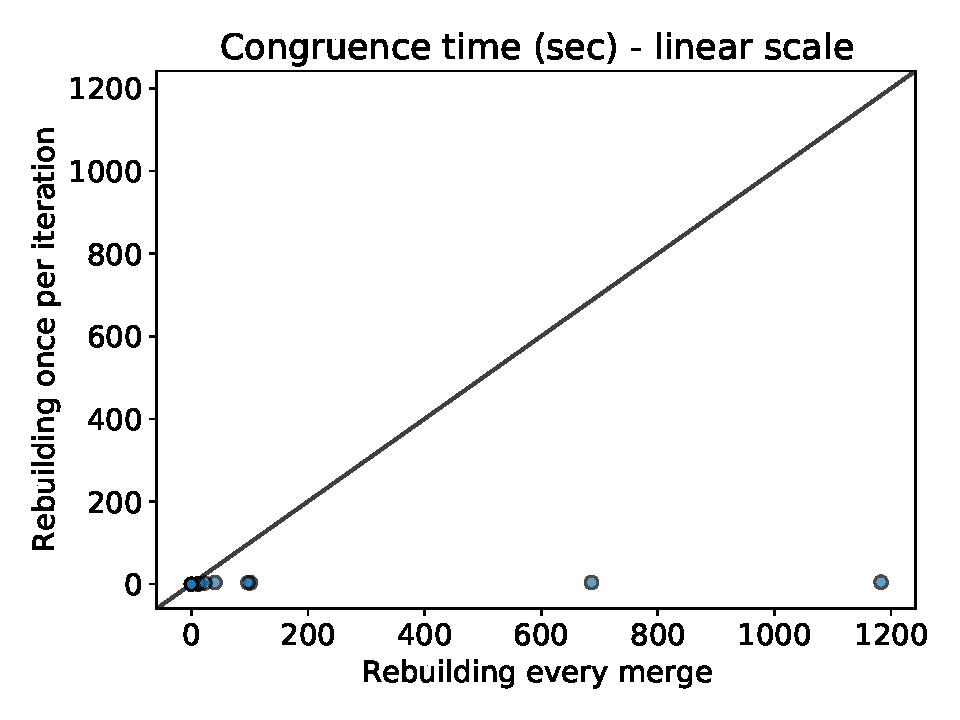
\includegraphics[height=5cm]{speedup}
  \end{subfigure}
  \hfill
  \begin{subfigure}{0.49\linewidth}
    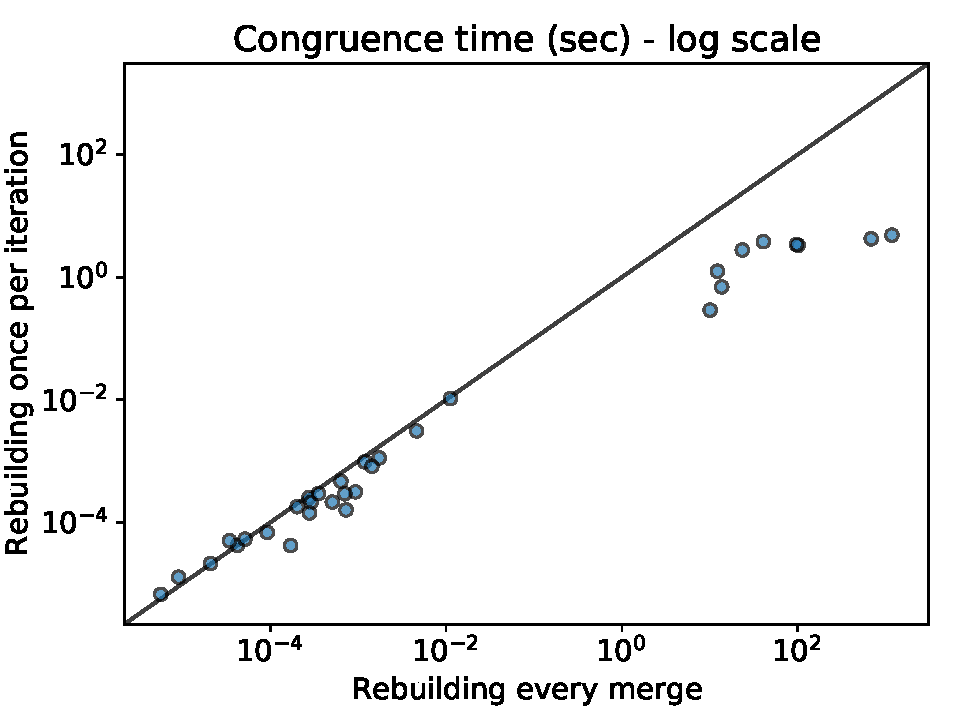
\includegraphics[height=5cm]{speedup-log}
  \end{subfigure}
  \caption{
    % 本段翻译未仔细校对
    % Rebuilding once per iteration---as opposed to after every merge---significantly
    %   speeds up congruence maintenance.
    % Both plots show the same data: one point for each of the \nEggTests tests.
    % The diagonal line is $y=x$;
    %   points below the line mean deferring rebuilding is faster.
    % In aggregate over all tests (using geometric mean),
    %   congruence is \CongrSpeedup faster, and
    %   equality saturation is \TotalSpeedup faster.
    % The linear scale plot shows that deferred rebuilding is significantly faster.
    % The log scale plot suggests the speedup is greater than some constant multiple;
    %   \autoref{fig:eval-iter} demonstrates this in greater detail.
    每次迭代只重建一次——而不是每次合并后——可显著加快同构维护。
    两个图显示相同的数据: 每个 \nEggTests 测试一个点。
    对角线是 $y=x$; 点在线下面意味着推迟重建更快。
    在所有测试中的总和(使用几何平均值), 同构快 \CongrSpeedup,等式饱和快 \TotalSpeedup。
    线性尺度图显示推迟重建显著更快。
    对数尺度图表明加速比某些常数倍大; 
      \autoref{fig:eval-iter}更详细地展示这一点。
  }
  \label{fig:eval}

  \begin{minipage}[t]{0.48\linewidth}
  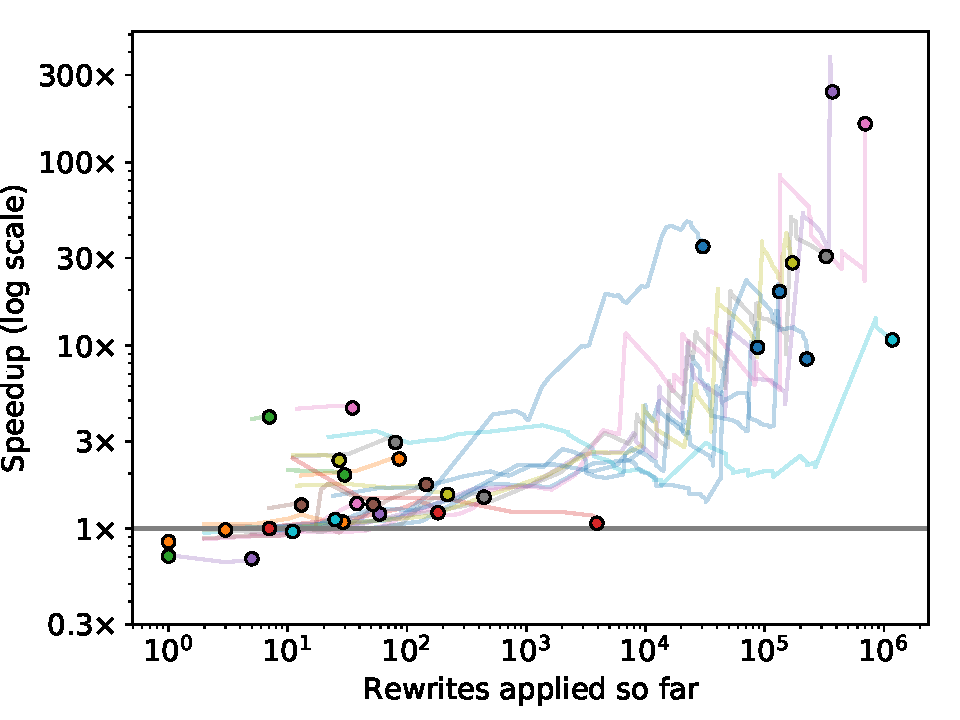
\includegraphics[height=5cm]{speedup-iter}
  \caption{
    % 本段翻译未仔细校对
    % As more rewrites are applied, deferring rebuilding gives greater speedup.
    % Each line represents a single test: each equality saturation iteration plots
    %   the cumulative rewrites applied so far against the multiplicative speedup
    %   of deferring rebuilding; the dot represents the end of that test.
    % Both the test suite as a whole (the dots) and individual tests (the lines)
    %   demonstrate an asymptotic speedup that increases with
    %   the problem size.
    当应用更多重写时,推迟重建会带来更大的加速。
    每条线表示一个测试:
      每次等式饱和迭代绘制目前已经应用的累计重写与推迟重建的乘法加速率; 
      点表示该测试结束。
    整个测试套件(点)和单独的测试(线)均表明随着问题规模的增大而增加的渐近加速。
  }
  \label{fig:eval-iter}
  \end{minipage}
  \hfill
  \begin{minipage}[t]{0.48\linewidth}
  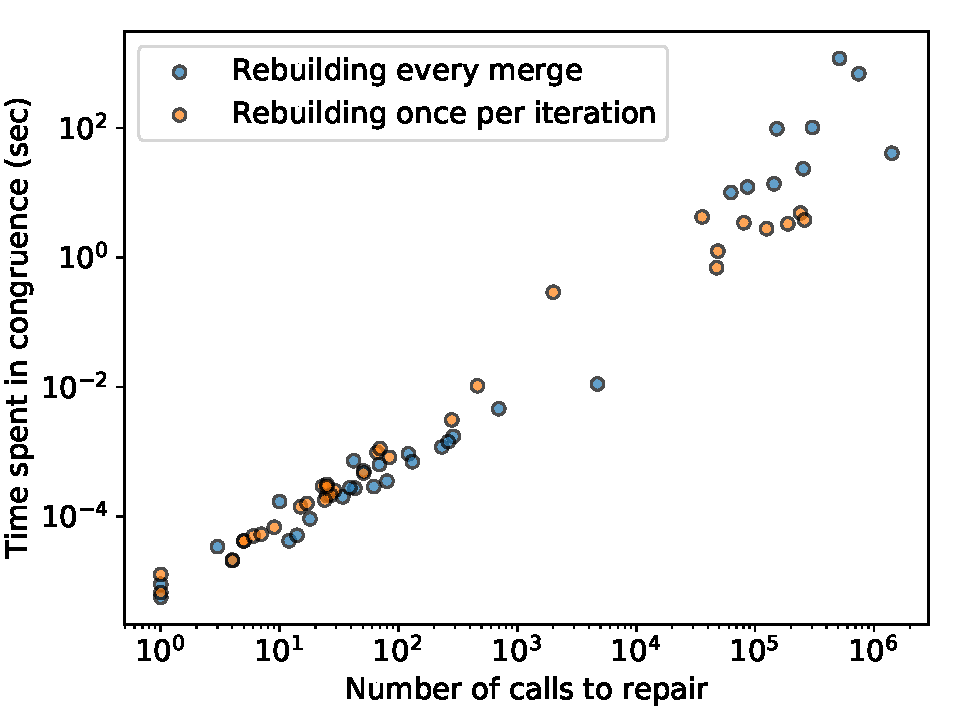
\includegraphics[height=5cm]{repairs}
  \caption{
    % 本段翻译未仔细校对
    % The time spent in congruence maintenance correlates with the number of calls
    % to the \texttt{repair} method.
    % Spearman correlation yields $r=\RepairsR$ with a p-value of \RepairsP,
    % indicating that the two quantities are indeed positively correlated.
    同构维护中的时间与\texttt{repair}方法的调用次数相关。
    Spearman 相关系数为 $r=\RepairsR$,p值为 \RepairsP,
      表明这两个量确实是正相关的。
  }
  \label{fig:repair-plot}
  \end{minipage}
\end{figure}


% 本段翻译未仔细校对
% We ran \egg's test suite using both rebuild strategies, measuring the time spent
%   on congruence maintenance.
% Each test consists of one run of \egg's equality saturation algorithm to optimize
%   a given expression.
% Of the \nEggTests total tests,
%   \nEggTimeouts hit the iteration limit of 100 and the remainder saturated.
% Note that both rebuilding strategies use \egg's phase-split equality saturation
%   algorithm, and the resulting \egraphs are identical in all cases.
% These experiments were performed on a 2020 Macbook Pro with a 2 GHz quad-core
%   Intel Core i5 processor and 16GB of memory.
我们使用两种重建策略运行了 \egg 的测试套件,并测量了在同余维护上花费的时间。
每个测试都包括一次 \egg 的等式饱和算法,以优化给定表达式。
在总共 \nEggTests 的测试中,
\nEggTimeouts 达到了100次迭代的限制,其余达到了饱和状态。
请注意,两种重建策略均使用 \egg 的分阶段等式饱和算法,并且所有情况下的 \egraphs 都是相同的。
这些实验在带有 2 GHz 四核 Intel Core i5 处理器和 16GB 内存的 2020 Macbook Pro 上进行。

% 本段翻译未仔细校对
% \autoref{fig:eval} shows our how rebuilding speeds up congruence maintenance.
% Overall, our experiments show an aggregate \CongrSpeedup speedup on congruence
%   closure and \TotalSpeedup speedup over the entire equality saturation
%   algorithm.
% \autoref{fig:eval-iter} shows this speedup is asymptotic;
%   the multiplicative speedup increases as problem gets larger.
图 \autoref{fig:eval} 显示了重建如何加速同余维护。
总体而言,我们的实验显示整体上同余闭包上有 \CongrSpeedup 加速,
  整个等式饱和算法上有 \TotalSpeedup 加速。
图 \autoref{fig:eval-iter} 显示这种加速是渐近的,随着问题规模变得更大,乘法加速率增加。


% \egg's test suite consists of two main applications:
% \texttt{math},
%   a small computer algebra system capable of symbolic differentiation and
%   integration; and
% \texttt{lambda},
%   a partial evaluator for the untyped lambda calculus using explicit
%   substitution to handle variable binding (shown in \autoref{sec:impl}).
% Both are typical \egg applications primarily driven by
%   syntactic rewrites, with a few key uses of \egg's more complex features
%   like \eclass analyses and dynamic/conditional rewrites.
\egg 的测试套件由两个主要应用组成:
\texttt{math},
一个小型计算机代数系统,能够进行符号导数和积分;
\texttt{lambda},
  一个无类型 lambda 演算的部分解释器,使用显式替换来处理变量绑定
  (如 \autoref{sec:impl} 所示)。
这两者都是典型的 \egg 应用,主要由语法重写驱动,
  并使用了 \egg 复杂的关键功能,如 \eclass 分析和动态或条件重写。


% \egg can be configured to capture various metrics about equality saturation as
%   it runs, including the time spent in the read phase (searching for matches),
%   the write phase (applying matches), and rebuilding.
% In \autoref{fig:eval}, congruence time is measured as the time spent
%   applying matches plus rebuilding.
% Other parts of the equality saturation algorithm (creating the initial \egraph,
%   extracting the final term) take negligible take compared to the equality
%   saturation iterations.
可以配置 \egg 来捕获运行过程中等式饱和的各种度量,
  包括读取阶段(搜索匹配)、写入阶段(应用匹配)和重建阶段的花费时间。
在 \autoref{fig:eval} 中,同余时间被测量为应用匹配和重建的时间。  % 同余? 下面的同余也有疑问
等式饱和算法的其他部分(创建初始 \egraph,提取最终项)与等式饱和迭代相比花费非常小。


% Deferred rebuilding amortizes the examination of \eclasses
%   for congruence maintenance;
%   deduplicating the worklist reduces the number of calls to the \texttt{repair}.
% \autoref{fig:repair-plot} shows that time spent in congruence is correlated with
%   the number of calls to the \texttt{repair} methods.
推迟重建对 \eclasses 的同余维护检查进行了摊销;
  去重工作列表减少了对 \texttt{repair} 的调用次数。
\autoref{fig:repair-plot} 显示,同余中的时间与\texttt{repair}方法的调用次数相关。


% The case study in \autoref{sec:herbie} provides a further evaluation of
%   rebuilding. Rebuilding (and other \egg features) have also been implemented in
%   a Racket-based \egraph, demonstrating that rebuilding is a conceptual advance
%   that need not be tied to the \egg implementation.
在 \autoref{sec:herbie} 中的案例研究进一步评估了重建。
  重建(和其他 \egg 特性)也已经在基于 Racket 的 \egraph 中实现,
  演示重建是为了概念推进,不用与 \egg 实现相关联。 %?

%%% Local Variables:
%%% TeX-master: "egg"
%%% End:
